\documentclass[border=3pt,tikz]{standalone}
\usepackage{tikz}
\usetikzlibrary{shapes.geometric, arrows, calc, positioning}

\colorlet{myred}{red!80!black}
\colorlet{myblue}{blue!80!black}
\colorlet{mygreen}{green!60!black}
\colorlet{myorange}{orange!70!red!60!black}
\colorlet{mydarkred}{red!30!black}
\colorlet{mydarkblue}{blue!40!black}
\colorlet{mydarkgreen}{green!30!black}


\tikzstyle{startstop} = [rectangle, rounded corners, minimum width=3cm, minimum height=1cm,text centered, draw=black, fill=green!30]
\tikzstyle{process} = [rectangle, minimum width=3cm, minimum height=1cm, text centered, draw=black, fill=pink!30]
\tikzstyle{arrow} = [thick,->,>=stealth]
\tikzstyle{residual} = [draw=blue!50, fill=blue!20, rectangle, rounded corners, minimum height=0.6cm]

\begin{document}

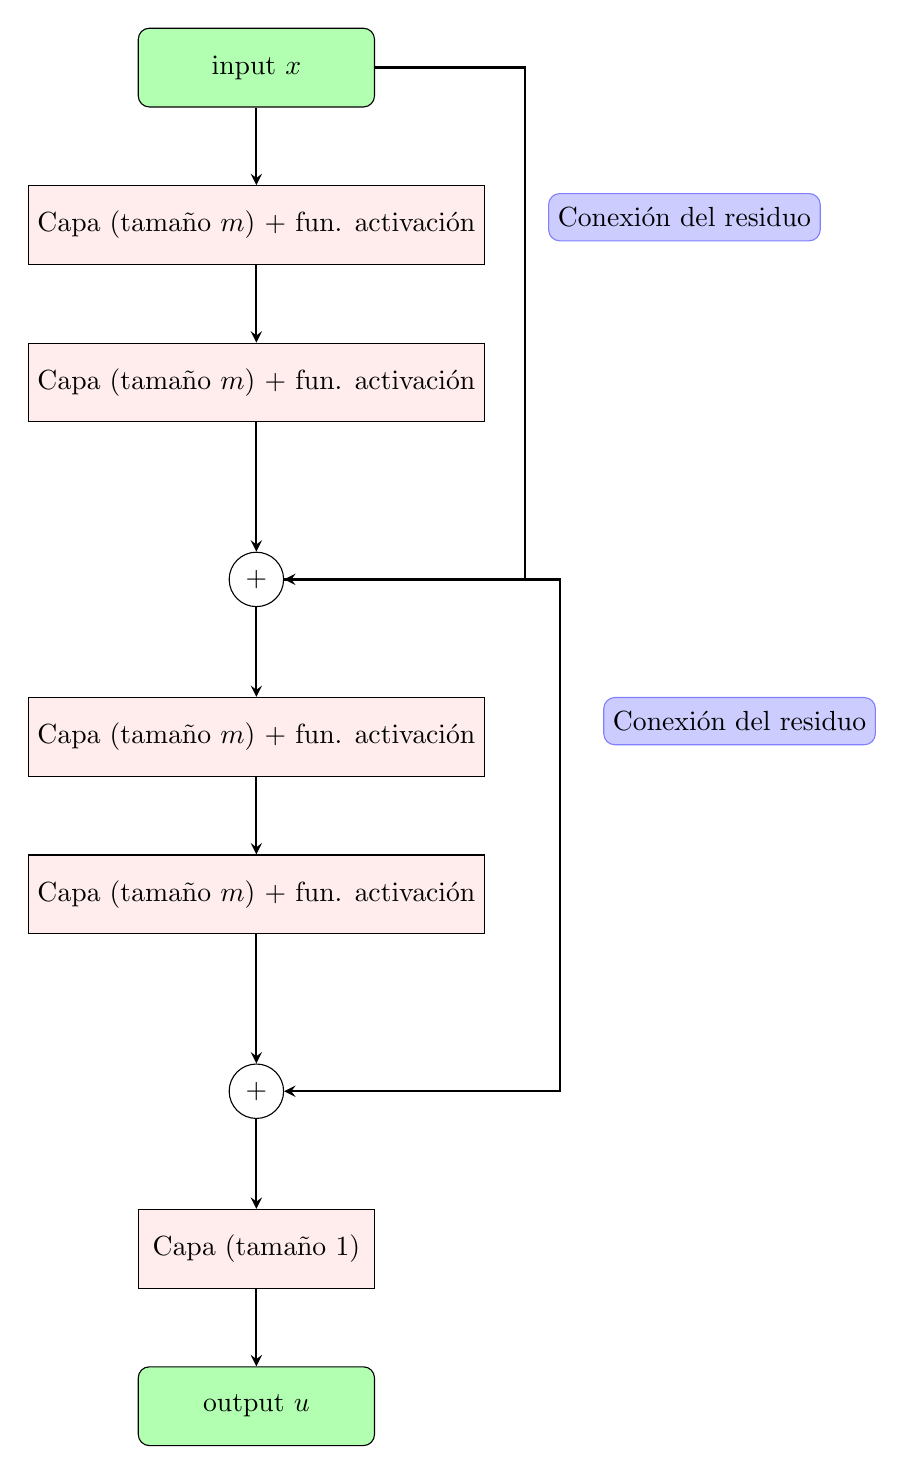
\begin{tikzpicture}[node distance=2cm]

% Nodes
\node (input) [startstop] {input $x$};
\node (fc1) [process, below of=input] {Capa (tamaño $m$) + fun. activación};
\node (fc2) [process, below of=fc1] {Capa (tamaño $m$) + fun. activación};
\node (add1) [circle, draw, below of=fc2, yshift=-0.5cm] {+};

\node (fc3) [process, below of=add1] {Capa (tamaño $m$) + fun. activación};
\node (fc4) [process, below of=fc3] {Capa (tamaño $m$) + fun. activación};
\node (add2) [circle, draw, below of=fc4, yshift=-0.5cm] {+};

\node (fc5) [process, below of=add2] {Capa (tamaño 1)};
\node (output) [startstop, below of=fc5] {output $u$};

% Arrows
\draw [arrow] (input.south) -- ++(0,-0.5) -| (fc1.north);
\draw [arrow] (fc1.south) .. controls +(0,-1) and +(0,1) .. (fc2.north);
\draw [arrow] (fc2.south) -- ++(0,-0.5) -- (add1.north);

\draw [arrow] (add1.south) .. controls +(0,-1) and +(0,1) .. (fc3.north);
\draw [arrow] (fc3.south) .. controls +(0,-1) and +(0,1) .. (fc4.north);
\draw [arrow] (fc4.south) -- ++(0,-0.5) -- (add2.north);

\draw [arrow] (add2.south) .. controls +(0,-1) and +(0,1) .. (fc5.north);
\draw [arrow] (fc5.south) -- (output.north);

% Residual connections
\draw [arrow] (input.east) -- ++(1.9cm,0) |- ($(add1.east)$);
\node[residual, anchor=west] at ($(fc1.east) + (0.8cm,0.1)$) {Conexión del residuo};

\draw [arrow] (add1.east) -- ++(3.5cm,0) |- ($(add2.east)$);
\node[residual, anchor=west] at ($(fc3.east) + (1.5cm,0.2)$) {Conexión del residuo};

\end{tikzpicture}

\end{document}
